\documentclass[a4,semhelv,semrot,portrait]{seminar}
\usepackage{graphicx}
\usepackage{fancybox}
\usepackage{a4wide}
\usepackage{amsmath}
\usepackage{amsxtra}

\newcommand{\mb}[1]{\mathbf{#1}}
\newcommand{\ket}[1]{|#1 \rangle}
\newcommand{\bra}[1]{\langle #1|}
\newcommand{\Alpha}{\bar{\alpha}}
\newcommand{\Exp}[2]{e^{i \mb{#1} \cdot \mb{#2} }}
\newcommand{\ExpM}[2]{e^{-i \mb{#1} \cdot \mb{#2} }}
\newcommand{\state}[2]{\psi_{#1 #2}}
\newcommand{\Muq}{\mu(\mb{q},\theta,\phi)}
\newcommand{\Angstrom}{\stackrel{\circ}{\mathrm{A}} }
\newcommand{\InvAngstrom}{ \stackrel{\circ}{\mathrm{A}}^{-1} } 
\newcommand{\Half}{\frac{1}{2}}

\slideframe{shadow}

\newcommand{\heading}[1]{ \begin{center}%
                          {\Large {\bf \sffamily{#1}}}\\[4mm]%
                          \hrule\vspace{1mm}
                          \end{center}}
\sffamily

\begin{document}

\begin{slide*}
    \begin{center}
    
\includegraphics[width=1.5cm]{UMCrest97.eps}\\[10mm]
    {\bf \Large Investigation of Theoretical Approaches for 
    Computing Relativistic Atomic Form Factors}\\[10mm]
    \hrule
    \vspace{10mm}
    {\large Michael Papasimeon \\
    Supervisor : Dr. Christopher Chantler \\
    Optics Group, School of Physics \\
    The University of Melbourne}
    \end{center}
\end{slide*}

\begin{slide*}
    \heading{OUTLINE}
    \begin{itemize}
        \item Project Overview
        \item Atomic Form Factor Theory
        \item Summary of Project Work and Results
        \item Further Work
    \end{itemize}
\end{slide*}

\begin{slide*}
    \heading{MOTIVATION}
    \begin{itemize}
        \item Applications
        \begin{itemize}
            \item Crystallography and Materials Science
            \item Medicine
            \item Astronomy
        \end{itemize}
        \item Existing Theoretical and Experimental Results
        \begin{itemize}
            \item Chantler
            \item Kissel and Pratt
            \item Cromer and Libermann
            \item Creagh
            \item Hubbell
            \item Scofield
            \item Henke
        \end{itemize}
    \end{itemize}
\end{slide*}

\begin{slide*}
    \heading{PROJECT AIMS}
    \begin{itemize}
        \item Aim 1
    \end{itemize}
\end{slide*}

\begin{slide*}
    \heading{ATOMIC FORM FACTOR THEORY}
    \begin{itemize}
        \item Total Form Factor
        \[
            f = f_0 + f' + if''
        \]
        \item Normal Form Factor
        \[
             f_0(q) = \int \rho(\mb{r}) e^{i\mb{q}\cdot\mb{r}} \; d\mb{r}
        \]
        \[
            q = |\mb{k_{final}} - \mb{k_{initial}}| = \frac{4\pi \sin(\theta/2)}{\lambda}
            \InvAngstrom
        \]
        \item Anomalous Form Factor
        \[
             f''(\omega) = \frac{\omega}{4\pi c r_0} \sigma(\omega)
        \]
        \item Dispersion Relation for $f'(\omega)$
        \[
             f'(\omega) = f'(\infty) - \frac{2}{\pi} P
                 \int_0^\infty 
                 \frac{\omega' f''(\omega')}{\omega^2 - {\omega'}^2} \; d\omega'
        \]
    \end{itemize}
\end{slide*}

\begin{slide*}
    \heading{THEORETICAL LIMITATIONS AND ASSUMPTIONS}
    \begin{itemize}
        \item Atomic Structure
        \item Electromagnetic Field
        \item Isolated Atom
        \item Perturbation Theory
        \item Additional Processes
            \begin{itemize}
                \item Photoionisation and Bound-Bound Transitions
                \item Rayleigh, Compton and Delbr\"uck Scattering
                \item Pair Production, Nuclear Thomson Scattering
            \end{itemize}
        \item Numerical and Computational Issues
    \end{itemize}
\end{slide*}

\begin{slide*}
    \heading{NORMAL FORM FACTOR FOR HYDROGENIC ATOMS}
    \begin{itemize}
        \item Non Relativistic (Schr\"odinger Wavefunctions)
        \[
             f_0(q) = \left( \frac{2Z}{a_0} \right)^4 
                     \left[ \left( \frac{2Z}{a_0} \right)^2 + q^2 \right]^{-2} 
        \]
        \item Relativistic Result (Dirac 4 Component Spinors)
        \[
        \begin{split}
              f_0(q) = 
            \frac{\Gamma(2\gamma_1)}{2iq \Gamma(2\gamma_1+1)}
            \left(
                \frac{2Z}{a_0}
            \right)^{2\gamma_1 + 1} \times \\
            \left[
                \frac{
                    \left(
                        \frac{2Z}{a_0} + iq
                    \right)^{2\gamma_1}
                    -
                    \left(
                        \frac{2Z}{a_0} - iq
                    \right)^{2\gamma_1}
                } {
                    \left[
                        \left(
                            \frac{2Z}{a_0} 
                        \right)^2   
                        + q^2
                    \right]^{2\gamma_1}
                }
            \right]
        \end{split}
        \]
        \item $\gamma_1 = \sqrt{1 - (\alpha Z)^2}$
    \end{itemize}
\end{slide*}

\begin{slide*}
    \heading{ATOMIC HYDROGEN}
    \begin{center}
        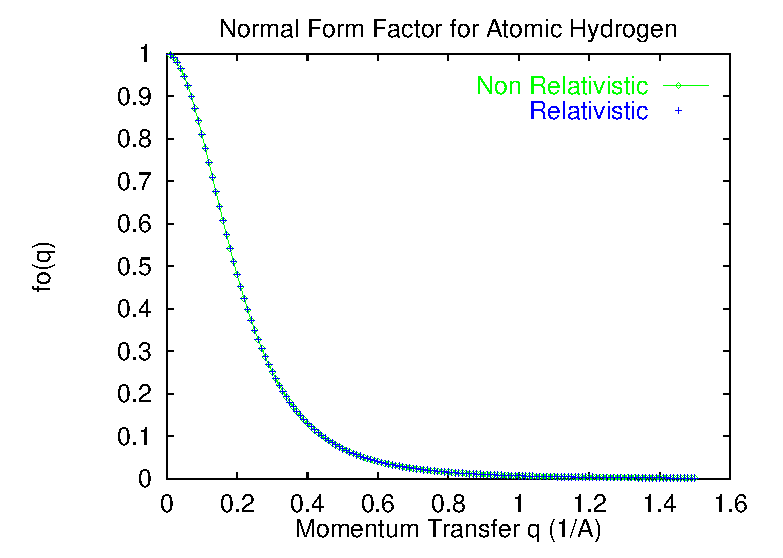
\includegraphics[height=6cm,angle=90]{f0_hydrogen.eps}
    \end{center}
\end{slide*}

\begin{slide*}
    \heading{HYDROGENIC URANIUM}
    \begin{center}
        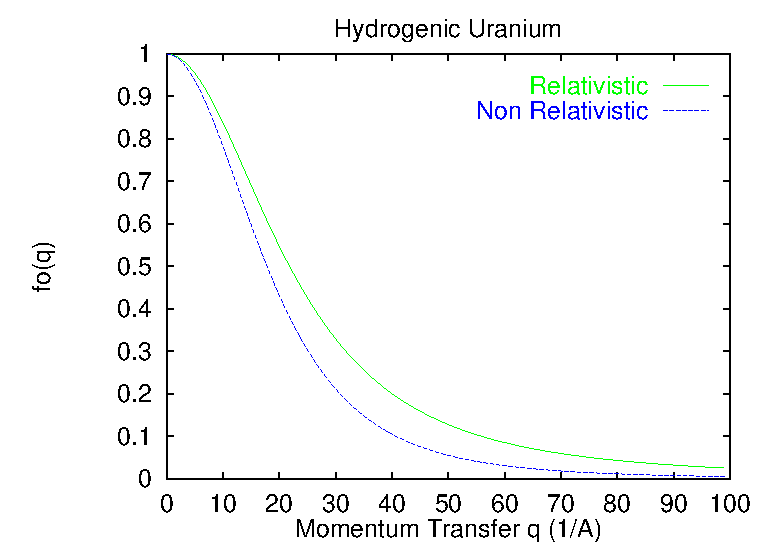
\includegraphics[height=6cm,angle=90]{f0_uranium.eps}
    \end{center}
\end{slide*}

\begin{slide*}
    \heading{$\Delta f_0(q)$ (Relativistic - Non Relativistic)}
    \begin{center}
        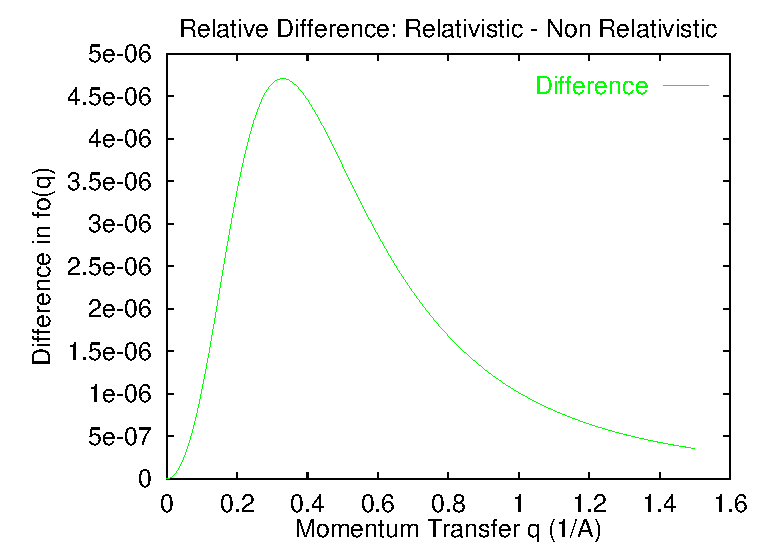
\includegraphics[height=6cm,angle=90]{delta_theory.eps}
    \end{center}
\end{slide*}

\begin{slide*}
    \heading{Comparing with Hubbell's Results}
    \begin{center}
        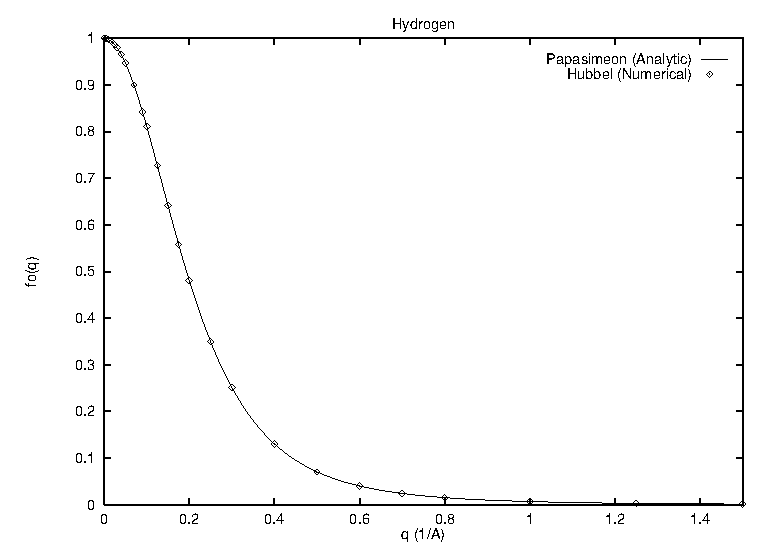
\includegraphics[height=4.5cm]{hubbel_papa.eps}
        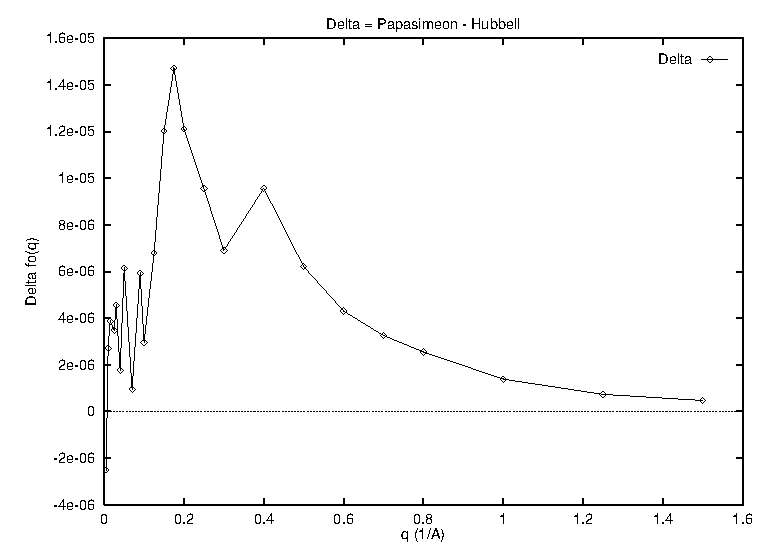
\includegraphics[height=4.5cm]{delta_hubbell.eps}
    \end{center}
\end{slide*}

\begin{slide*}
    \heading{Anomalous Atomic Form Factor}
    \begin{itemize}
        \item Approaches to Calculating $f''(\omega)$
        \begin{itemize}
            \item Standard Perturbation Theory
            \item Relativistic Perturbation Theory
            \item Relativistic S-Matrix Theory
        \end{itemize}
        \item Relativistic Emission and Absorption Operators
        \begin{eqnarray*} 
            \mathcal{A}_i       & = & \sum_j \Alpha \cdot \hat{\epsilon}_j \Exp{k_i}{r_j} \\
            \mathcal{A}_f^{\dag}   & = & \sum_j \Alpha \cdot \hat{\epsilon}_j \ExpM{k_f}{r_j}
        \end{eqnarray*}
        \item Relativistic Photoionisation Amplitude
            \begin{itemize}
                \item $A_1(k,k') = \bra{\psi_c} \mathcal{A}_i \ket{\psi_0} = \bra{\psi_c} \Exp{k}{r} \Alpha_j \ket{\psi_0}$
            \end{itemize}
    \end{itemize}
\end{slide*}

\begin{slide*}
    \heading{Photoionisation Coordinate System}
    \begin{center}
        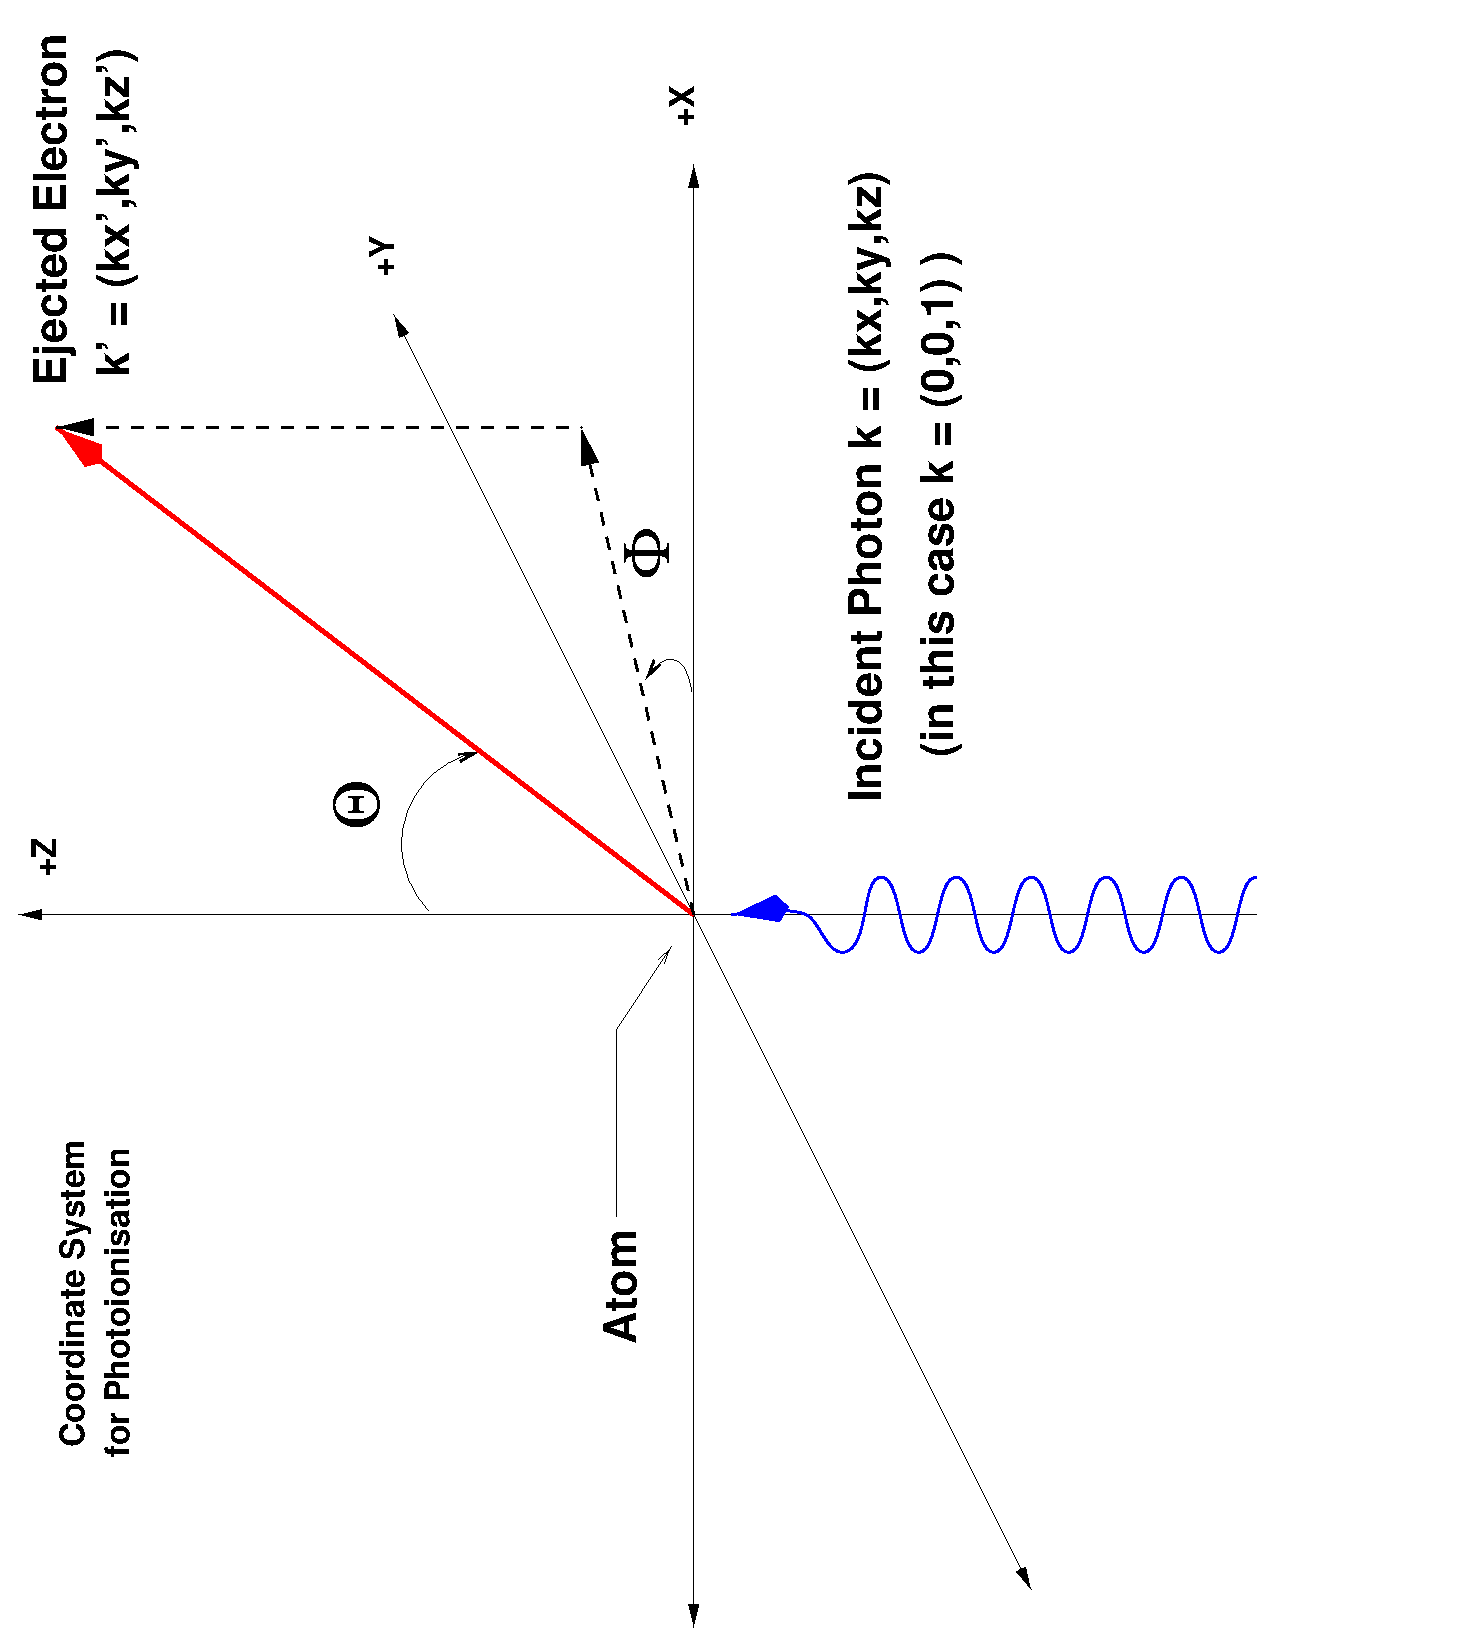
\includegraphics[width=6cm,angle=-90]{coords.eps}
        \[
        \begin{array}{cccc}
            k'_x & = & |k'| \sin(\Theta) \cos(\Phi) & \\
            k'_y & = & |k'| \sin(\Theta) \sin(\Phi) & \\
            k'_z & = & |k'| \cos(\Theta)&
          \end{array}
        \]
    \end{center}
\end{slide*}

\begin{slide*}
    \heading{All Poles Result}
    \[
    \begin{split}
     A_1(\mb{k},\mb{k'})_x =
    \frac{G_0 \Gamma(\gamma_1 + 2)}{\sqrt{4\pi}} 
    \int_{0}^{2\pi}
    \int_{0}^{\pi} \\
        \left[
            \frac {
            \sin(\theta) [ \xi(k'_x - ik'_y) + i F_0 \sin(\theta) e^{i\phi} ]
            } {
                (\frac{1}{2}\sigma_1 - i \Muq )^{\gamma_1 + 2}
            }
       \right]
    \; d\theta
    \; d\phi
    \end{split}
    \]
\end{slide*}

\end{document}
